
\chapter{TABLESAT ATTITUDE SOFTWARE IMPLEMENTATION}
\label{chap:TableSatAttitudeDynamicsSoftware}

\TODO{This chapter is just pulled out code snippets for now.  Will fill in text}

\section{Implementation of Attitude Modeling}
\label{sec:ImplementationofAttitudeModeling}


\subsection{Quaternion Notation}
\label{subsec:Implementation-QuaternionNotation}
Section \ref{subsubsec:QuaternionNotation}

As is described more in Chapter \ref{chap:TSatPy}, the implementation in this thesis is done in an object oriented manner so it can handle either the scalar first or scalar last format.

\begin{singlespace}
  \begin{minted}[mathescape,linenos,numbersep=10pt,frame=lines,framesep=2mm]{python}
from TSatPy.State import Quaternion
q = Quaternion(vector=[1,2,3], scalar=4)
print(q)
q = Quaternion(scalar=0, vector=[1,2,3])
print(q)

# Prints Out
# <Quaternion [1 2 3], 4>
# <Quaternion [1 2 3], 0>
  \end{minted}
  \nocite{minted}
\end{singlespace}

\section{Rotational Quaternion}
\label{sec:Implementation-RotationalQuaternion}
Section \ref{subsubsec:RotationalQuaternion}

Creating a rotational quaternion from the TSatPy (Chapter \ref{chap:TSatPy}) is done with

\begin{singlespace}
  \begin{minted}[mathescape,linenos,numbersep=10pt,frame=lines,framesep=2mm]{python}
from TSatPy.State import Quaternion

q = Quaternion(vector=[1,2,3], radians=4)
e, theta = q.to_rotation()

print(q)
print("Euler axis: <%g, %g, %g>" % (e[0,0], e[1,0], e[2,0]))
print("Rotation: %g radians" % theta)

# Prints Out
# <Quaternion [-0.24302 -0.48604 -0.72906], -0.416147>
# Euler axis: <-0.267261, -0.534522, -0.801784>
# Rotation: 4 radians
  \end{minted}
  \nocite{minted}
\end{singlespace}

\subsection{Quaternion Multiplication}
\label{subsec:Implementation-QuaternionMultiplication}

Section \ref{subsubsec:QuaternionMultiplication}

The example below shows how this incremental changes holds true with the TSatPy library.
\begin{singlespace}
  \begin{minted}[mathescape,linenos,numbersep=10pt,frame=lines,framesep=2mm]{python}
from TSatPy.State import Quaternion

a = Quaternion([1,2,3], radians=0.5)
b = Quaternion([1,2,3], radians=2)
print("a             = %s" % a)
print("a * a * a * a = %s" % (a * a * a * a))
print("b             = %s" % b)
# Prints Out
# a             = <Quaternion [-0.0661215 -0.132243 -0.198364], 0.968912>
# a * a * a * a = <Quaternion [-0.224893 -0.449785 -0.674678], 0.540302>
# b             = <Quaternion [-0.224893 -0.449785 -0.674678], 0.540302>
  \end{minted}
  \nocite{minted}
\end{singlespace}

Section \ref{subsubsec:QuaternionMultiplication} includes a small example of quaternion multiplication and the following snippet is the implementation of the quaternion multiplication which reads and is used similarly to how the quaternion algebra is written.

\begin{singlespace}
  \begin{minted}[mathescape,linenos,numbersep=10pt,frame=lines,framesep=2mm]{python}
class Quaternion(object):
    def __mul__(self, q):
        v = (self.x + np.eye(3) * self.scalar) * q.vector
        v += self.vector * q.scalar
        s = self.scalar * q.scalar - (self.vector.T * q.vector)[0, 0]
        return Quaternion(v, s)
  \end{minted}
  \nocite{minted}
\end{singlespace}


\subsection{Rotating a Point with Quaternions}
\label{subsubsec:RotatingaPointwithQuaternions}

One of the main focal points of this thesis is to ensure that the tools developed in this research aide in the further development of observer-based attitude control.  To enable this goal, ``run-time'' analysis of the system is critical.  Waiting for the completion of a simulation or experimental test with TableSat IA before being able to access the information is not only an impedance to this end, but it also introduces complexity and higher ``run-time'' costs to collect and store all simulation/experimental data.  Watching representation of the system's state change as the experiment runs provides valuable insight.  In the case of an estimator, sensor voltages are converted to a measured state and the observer attempts to use it to estimate the true state of the system.  A valuable visualization is both the measured and estimated states displayed in wireframe so the effectiveness of the estimator can be readily observed.  The points in a wireframe model of TableSat can be rotated to show the estimated orientation through the use of a 3x3 rotation matrix $\bs{R}_q$ defined as
\begin{equation}
  \bs{R}_q = (q_0^2 - \bs{v}^T \bs{v}) \bs{I} + 2 \bs{v} \bs{v}^T - 2 q_0 (\bs{v} \times)
  \label{eqn:RotationMatrix}
\end{equation}

For example, for a $\pi/2$ radian rotation about $\bs{\hat{e}} = 0\bs{i}+0\bs{j}+1\bs{k}$, the rotational quaternion as defined in Equation (\ref{eqn:RotationalQuaternionDefinition}) becomes $q = 0\bs{i}+0\bs{j}-1/\sqrt{2}\bs{k}+1/\sqrt{2}$.  With Equation (\ref{eqn:RotationMatrix}), the rotational matrix becomes

\begin{equation}
  \begin{aligned}
    \bs{R_q} & = \left[ (1/\sqrt{2})^2 - (1/\sqrt{2})^2 \right] \bs{I} + 2 \begin{bmatrix} 0 & 0 & 0 \\ 0 & 0 & 0 \\ 0 & 0 & 1/\sqrt{2} \end{bmatrix} - 2 \frac{1}{\sqrt{2}} \begin{bmatrix} 0 & 1/\sqrt{2} & 0 \\ -1/\sqrt{2} & 0 & 0 \\ 0 & 0 & 0 \\ \end{bmatrix} \\
      & = \begin{bmatrix} 0 & -1 & 0 \\ 1 & 0 & 0 \\ 0 & 0 & 1 \\\end{bmatrix}
  \end{aligned}
\end{equation}

For the visualization, a point $A (2, 4, -1)$ that is in the standard orientation of body axes aligned with the global reference frame can be drawn at the current estimated location.  That is,

\begin{equation}
  A' = \bs{R_q} A = \begin{bmatrix} 0 & -1 & 0 \\ 1 & 0 & 0 \\ 0 & 0 & 1 \\\end{bmatrix} \begin{bmatrix} 2 \\ 4 \\ -1 \end{bmatrix} = \begin{bmatrix} -4 \\ 2 \\ -1 \end{bmatrix}
\end{equation}

The equivalent TSatPy implementation of the point rotation equation (Equation \ref{eqn:RotationMatrix})
\begin{singlespace}
  \begin{minted}[mathescape,linenos,numbersep=10pt,frame=lines,framesep=2mm]{python}
from TSatPy.State import Quaternion
import numpy as np

A = np.mat([2, 4, -1]).T
q = Quaternion([0,0,1], radians=np.pi/2)

print(q.rmatrix * A)

# Prints out
# [[-4.]
#  [ 2.]
#  [-1.]]
  \end{minted}
  \nocite{minted}
\end{singlespace}


\subsection{Quaternion-based Attitude Visualization}
\label{subsubsec:QuaternionbasedAttitudeVisualization}

% One of the largest challenges with running both simulations and live control models is having access to meaningful representations of how the system is performing.  NSS simulations are generally performed through either running of m-file scripts and analyzing logged data in a batch format after the run, or using a NSS to produce line plots of values tracked during the simulation run.


The method for calculating the new position of a point from an initial position can be extended to a collection of points that create a wireframe for the TableSat model.  Once this base wireframe is defined, the estimated attitude of the system can be visualized.  That is, if the system's estimator determines that TableSat is at an attitude of $\bs{q} = -0.38\bs{i}-0.07\bs{j}+0.91\bs{k}+0.16$, for example, this is equivalent to a 161 degree rotation about the Euler axis $\bs{\hat{e}} = 0.3844\bs{i}+0.0708\bs{j}-0.9205\bs{k}$.  Figure \ref{fig:TSatWireframe} shows the TableSat wireframe in its default configuration with its body axes aligned with the global reference frame.  The red dashed line represents the axis of rotation.

% Ideally, generating and updating a rendered model of the system at simulation time can improve the ability to attain the desired system behavior.

\begin{figure}[H]
  \centerline{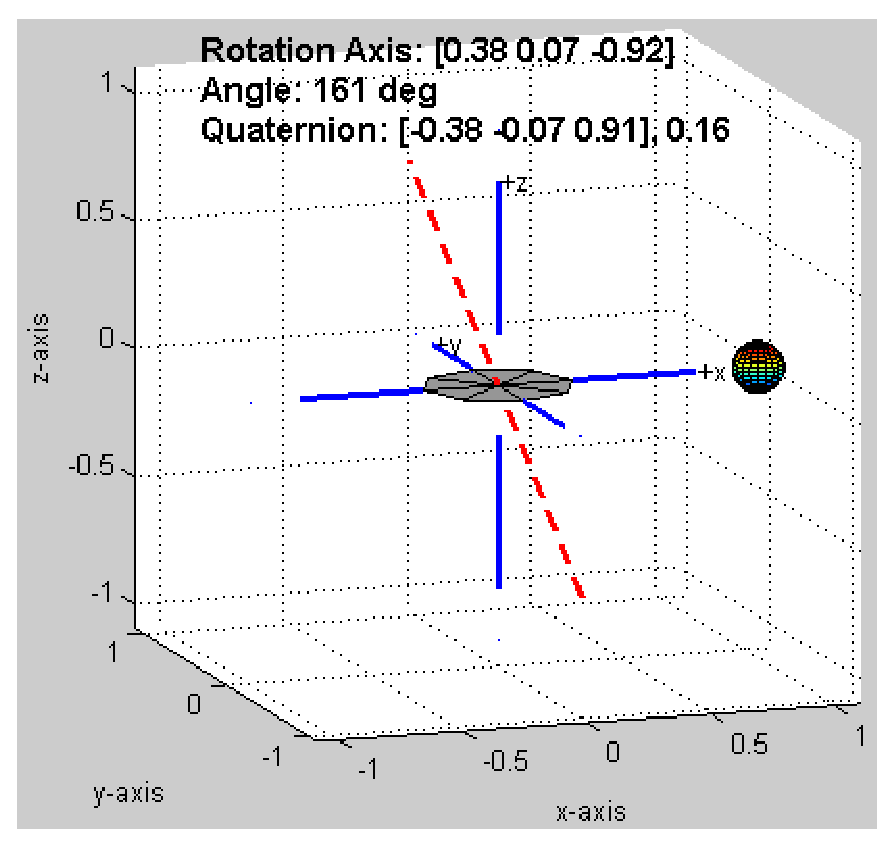
\psfig{file=figures/q_rotation_start.eps,height=3in}}
  \caption{TableSat Wireframe}
  \label{fig:TSatWireframe}
\end{figure}

Once new locations for all points in the wireframe are determined, it can be redrawn visualizing the estimated current orientation of the TableSat (Figure \ref{fig:TSatWireframeEstimatedAttitude}).  ``Run-time'' visualizations are discussed in greater detail in \TODO{Where did this end up??} to show how as the estimator is running, updates to the state estimate, $\bs{\hat{x}}$, can be used to update the wireframe's orientation.

\begin{figure}[H]
  \centerline{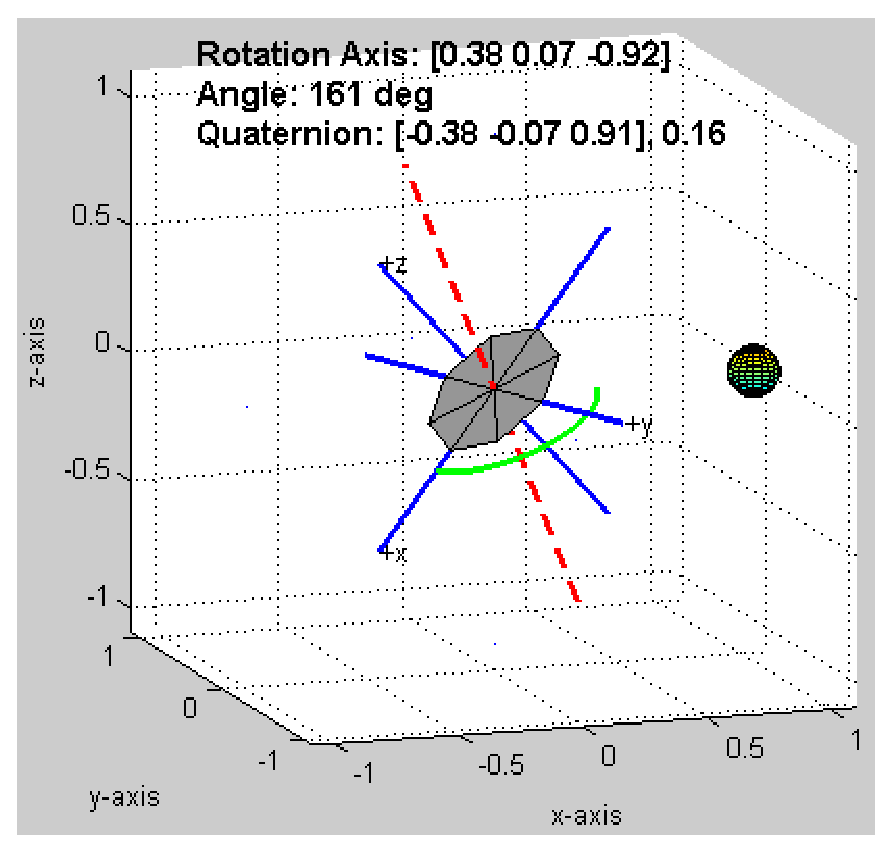
\psfig{file=figures/q_rotation_end.eps,height=3in}}
  \caption{TableSat Wireframe Estimated Attitude}
  \label{fig:TSatWireframeEstimatedAttitude}
\end{figure}


\subsection{Incremental Quaternion Rotations}
\label{subsubsec:IncrementalQuaternionRotations}

The quaternion's definition based on Euler's theorem of a rotation about a single axis simplifies the process of tracking the orientation of a spin-stabilized satellite.  NASA's MMS spacecraft has a mission spin rate of 3 rpm (~0.314 rad/sec).  A rotational quaternion, $\bs{q}_{rps}$, representing the per second rotation about the z-axis is

\begin{equation}
  \begin{aligned}
    \bs{q}_{rps} = & ( 0\bs{i} + 0\bs{j} + 1\bs{k} ) \sin \left( \frac{-0.314}{2} \right) + \cos \left( \frac{-0.314}{2} \right) \\
    = & 0\bs{i} +0\bs{j} -0.156434\bs{k} + 0.987688
  \end{aligned}
\end{equation}

In an open loop system, the best prediction of the state is to apply the quaternion rotation at each second to the previous steps state prediction, and the prediction is initialized with a known orientation.  For example, if TableSat performs a $+1/4$ turn about the z-axis each second, the best prediction at the current attitude can be obtained using just a quaternion multiplication as follows

\begin{equation}
  \begin{aligned}
    \bs{q}(t_{k+1}) = & \bs{q}_{rps} \otimes \bs{q}(t_{k}) \\
    \text{where } \bs{q}(t_0) = & 0 \bs{i} +0 \bs{j} -0.707107 \bs{k} +0.707107
  \end{aligned}
  \label{eqn:3rpmQuaternionEquation}
\end{equation}

Using the TSatPy code, Equation (\ref{eqn:3rpmQuaternionEquation}) can be implemented as

\begin{singlespace}
  \begin{minted}[mathescape,linenos,numbersep=10pt,frame=lines,framesep=2mm]{python}
from TSatPy.State import Quaternion
import time
import numpy as np

q_rps = Quaternion([0,0,1], radians=np.pi/10)
print('Quaternion spin rate (rad/sec)\n %s' % q_rps)

q_state = Quaternion([0,0,1], radians=np.pi/2)
print('Initial state of TableSat\n t=0: %s' % q_state)


print('Starting Open Loop State Tracking')
for k in range(1,11):
    time.sleep(1)
    q_state *= q_rps
    print(' t=%s: %s' % (k, q_state))

# Prints Out
# Quaternion spin rate (rad/sec)
#  <Quaternion [-0 -0 -0.156434], 0.987688>
# Initial state of TableSat
#  t=0: <Quaternion [-0 -0 -0.707107], 0.707107>
# Starting Open Loop State Tracking
#  t=1: <Quaternion [0 0 -0.809017], 0.587785>
#  t=2: <Quaternion [0 0 -0.891007], 0.45399>
#  t=3: <Quaternion [0 0 -0.951057], 0.309017>
#  t=4: <Quaternion [0 0 -0.987688], 0.156434>
#  t=5: <Quaternion [0 0 -1], 1.11022e-16>
#  t=6: <Quaternion [0 0 -0.987688], -0.156434>
#  t=7: <Quaternion [0 0 -0.951057], -0.309017>
#  t=8: <Quaternion [0 0 -0.891007], -0.45399>
#  t=9: <Quaternion [0 0 -0.809017], -0.587785>
#  t=10: <Quaternion [0 0 -0.707107], -0.707107>
  \end{minted}
  \nocite{minted}
\end{singlespace}

This implementation has both a significant theoretical and implementation issue.  The theoretical concern is the estimate is that running in an open loop fashion without receiving correction updates.  Therefore, the myriad of additional factors in a real system would quickly invalidate the accuracy of this approach.  The implementation issue deals with the time step.  Even if TableSat spins perfectly at 3 rpm, the state is not updated exactly on each second.  A busy processor, numerical drift, and execution time would prevent the desired fixed step size of 1 sec.  In some of the earlier implementations of the base station controller (discussed in Chapter \ref{chap:ProgressionOfControlSystemSoftware}), dropped UDP messages cause the control loop to execute on an inconsistent interval and prevent accurate state estimates.  (Handling of the variability in time steps is discussed in Section \ref{sec:SatelliteDynamics})


\subsection{Quaternion Decomposition}
\label{subsubsec:QuaternionDecomposition}

The attitude of TSat is represented by a single quaternion.  The change in attitude between two states can be modeled by the a rotation about a single axis.  Figure \ref{fig:PreDecomposedQuaternion} show the attitude of a system described by the quaternion $\bs{q} = [\alpha, \beta, \phi], 0.16953$ which is a rotation of 2.8 radians about the axis $[\alpha, \beta, \phi]^T$.  For control purposes, decomposing the single quaternion into one representing a rotation about the z-axis and a second rotation about an axis in the x-y plane as shown in Figure \ref{fig:PostDecomposedQuaternion}.

\begin{figure}[H]
  \begin{subfigure}[h!]{0.5\textwidth}
    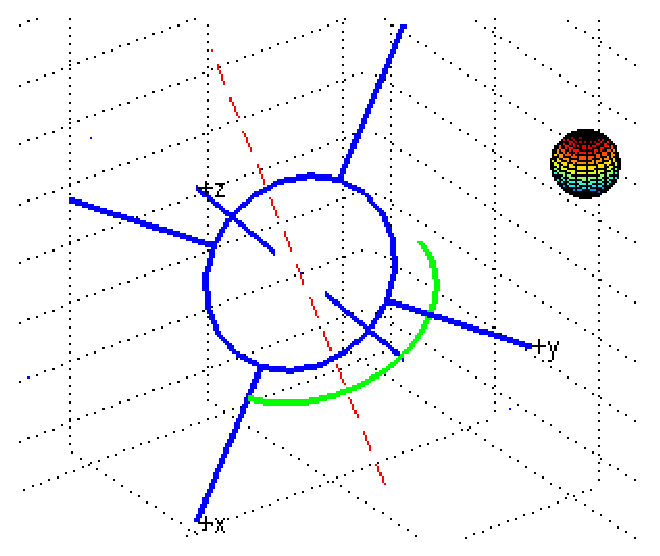
\includegraphics[width=\textwidth]{figures/quaternion_decompose_pre.eps}
    \caption{Quaternion State}
    \label{fig:PreDecomposedQuaternion}
  \end{subfigure}
  ~
  \begin{subfigure}[h!]{0.5\textwidth}
    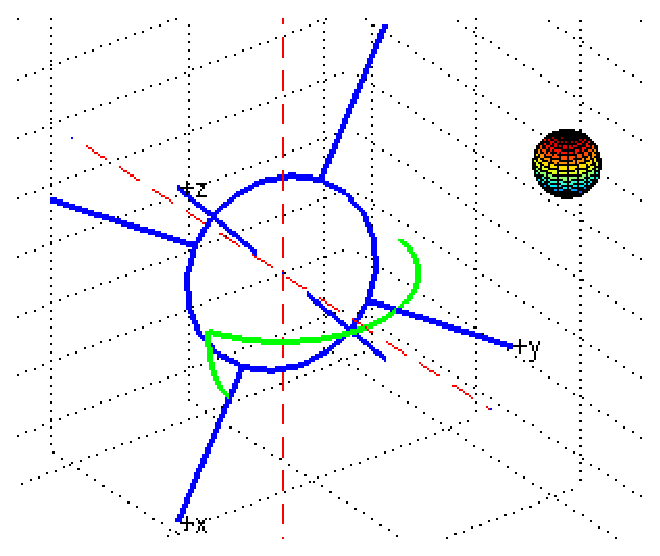
\includegraphics[width=\textwidth]{figures/quaternion_decompose_post.eps}
    \caption{Decomposed State}
    \label{fig:PostDecomposedQuaternion}
  \end{subfigure}
  \caption{Decomposing a Quaternion into Rotation and Nutation}
  \label{fig:QuaternionDecomposition}
\end{figure}

The quaternion that describes TSat's attitude $\bs{q}$ can be written as a sequence of two rotations.  A quaternion rotation about the z-axis $\bs{q_r}$ followed by the quaternion rotation about an axis in the x-y plane that creates a nutation $\bs{q_n}$.  Resultant rotations are performed through a left quaternion multiplication.
\begin{equation}
  \bs{q} = \bs{q_n} \otimes \bs{q_r} = \begin{bmatrix} \bs{v}_n \\ q_{0n} \end{bmatrix} \otimes \begin{bmatrix} \bs{v}_r \\ q_{0r} \end{bmatrix}
\end{equation}
\begin{equation}
  \begin{bmatrix}\bs{v} \\ q_{0} \end{bmatrix} =
  \begin{bmatrix} \bs{v}_n q_{0r} + \bs{v}_r q_{0n} + \bs{v}_n \times \bs{v}_r \\  q_{0n} q_{0r} - \bs{v}_n \cdot \bs{v}_r \end{bmatrix}
  \label{eqn:rot_nut_product}
\end{equation}
Expanding the vector components out creates the equation.
\begin{equation}
  \begin{bmatrix}
    q_{1} \\
    q_{2} \\
    q_{3} \\
    q_{0}
  \end{bmatrix}
  =
  \begin{bmatrix}
    \begin{bmatrix}
      q_{1n} \\
      q_{2n} \\
      q_{3n} \\
    \end{bmatrix} q_{0r} + \begin{bmatrix}
      q_{1r} \\
      q_{2r} \\
      q_{3r} \\
    \end{bmatrix} q_{0n} + \begin{bmatrix}
      q_{1n} \\
      q_{2n} \\
      q_{3n} \\
    \end{bmatrix} \times \begin{bmatrix}
      q_{1r} \\
      q_{2r} \\
      q_{3r} \\
    \end{bmatrix}
    \\
    q_{0n} q_{0r} - \begin{bmatrix}
      q_{1n} \\
      q_{2n} \\
      q_{3n} \\
    \end{bmatrix} \cdot \begin{bmatrix}
      q_{1r} \\
      q_{2r} \\
      q_{3r} \\
    \end{bmatrix} \\
  \end{bmatrix}
\end{equation}
and through simplification becomes
\begin{equation}
  \begin{bmatrix}
    q_{1} \\
    q_{2} \\
    q_{3} \\
    q_{0}
  \end{bmatrix}
  =
  \begin{bmatrix}
    q_{1n} q_{0r} + q_{1r} q_{0n} + q_{2n} q_{3r} - q_{3n} q_{2r} \\
    q_{2n} q_{0r} + q_{2r} q_{0n} + q_{3n} q_{1r} - q_{1n} q_{3r} \\
    q_{3n} q_{0r} + q_{3r} q_{0n} + q_{1n} q_{2r} - q_{2n} q_{1r} \\
  q_{0n} q_{0r} - (q_{1n} q_{1r} + q_{2n} q_{2r} + q_{3n} q_{3r} ) \\
  \end{bmatrix}
  \label{eqn:rot_nut_product_simplified}
\end{equation}
Now that we have an expanded representation of the resultant quaternion, we can use the restriction from the desired spin-stabilized state for TableSat.  The rotational quaternion is allowed to move freely about the $z$-axis but should not have any displacement about the $x$ and $y$ axes.  From Equation \ref{eqn:RotationalQuaternionDefinition}, $q_{1r} = q_{2r} = 0$.
\begin{equation}
  \bs{q_{r}}
  = q_{1r} \bs{i} + q_{2r} \bs{j} + q_{3r} \bs{k} + q_{0r}
  = 0 \bs{i} + 0 \bs{j} + q_{3r} \bs{k} + q_{0r}
  \label{eqn:rotation_quaternion_defined}
\end{equation}
The nutation quaternion has the opposite restrictions where rotation is allowed about the $x$ and $y$ axes but not about the $z$ axis.  From Equation \ref{eqn:RotationalQuaternionDefinition}, $q_{3n} = 0$.
\begin{equation}
  \bs{q_{n}}
  = q_{1n} \bs{i} + q_{2n} \bs{j} + q_{3n} \bs{k} + q_{0n}
  = q_{1n} \bs{i} + q_{2n} \bs{j} + 0 \bs{k} + q_{0n}
  \label{eqn:nutation_quaternion_defined}
\end{equation}
Substituting equations \eqref{eqn:rotation_quaternion_defined} and \eqref{eqn:nutation_quaternion_defined} into \eqref{eqn:rot_nut_product_simplified} yields.
\begin{equation}
  \begin{bmatrix}
    q_{1} \\
    q_{2} \\
    q_{3} \\
    q_{0}
  \end{bmatrix}
  =
  \begin{bmatrix}
    q_{1n} q_{0r} + 0             + q_{2n} q_{3r} - 0 \\
    q_{2n} q_{0r} + 0             + 0             - q_{1n} q_{3r} \\
    0             + q_{3r} q_{0n} + 0             - 0 \\
  q_{0n} q_{0r} - (q_{1n} 0 + q_{2n} 0 + 0 q_{3r} ) \\
  \end{bmatrix}
\end{equation}
\begin{subequations}
  \begin{align}
    q_{1} &= q_{1n} q_{0r} + q_{2n} q_{3r} \label{eqn:rot_nut_1_1} \\
    q_{2} &= q_{2n} q_{0r} - q_{1n} q_{3r} \label{eqn:rot_nut_1_2} \\
    q_{3} &= q_{3r} q_{0n} \label{eqn:rot_nut_1_3} \\
    q_{0} &= q_{0n} q_{0r} \label{eqn:rot_nut_1_0}
  \end{align}
\end{subequations}
Solving \ref{eqn:rot_nut_1_3} and \ref{eqn:rot_nut_1_0} for $q_{3r}$ and $q_{0r}$ and substituting into \ref{eqn:rot_nut_1_1} and \ref{eqn:rot_nut_1_2}
\begin{subequations}
  \begin{align}
    q_{0n} q_{1} &= q_{1n} q_{0} + q_{2n} q_{3} \label{eqn:rot_nut_2_1} \\
    q_{0n} q_{2} &= q_{2n} q_{0} - q_{1n} q_{3} \label{eqn:rot_nut_2_2}
  \end{align}
\end{subequations}
combining \ref{eqn:rot_nut_2_1} and \ref{eqn:rot_nut_2_2}
\begin{equation}
  0 = (q_{0}q_{2} + q_{1}q_{3}) q_{1n} + (q_{2}q_{3} - q_{0}q_{1}) q_{2n}
\end{equation}
\begin{subequations}
  \begin{align}
    q_{1n} &= Q \cdot q_{2n} \\
    \text{where } Q &= \frac{q_{0}q_{1} - q_{2}q_{3}}{q_{0}q_{2} + q_{1}q_{3}}
  \end{align}
  \label{eqn:nutation_parameter_ratio}
\end{subequations}
The additional restriction than rotational quaternions have a unit norm can be leveraged in finding solutions
\begin{equation}
  \left\| \bs{q} \right\| = \sqrt{\bs{v} \cdot \bs{v} + q_0^2} = \sqrt{q_1^2+q_2^2+q_3^2+q_0^2}
  \label{eqn:quaternion_norm}
\end{equation}
Taking the norm of the rotational quaternion in Equation \ref{eqn:rotation_quaternion_defined} and substituting $q_{3r}$ and $q_{0r}$ from Equations \ref{eqn:rot_nut_1_3} and \ref{eqn:rot_nut_1_0} becomes
\begin{equation}
  (0)^2 + (0)^2 + \left( \frac{q_3}{q_{0n}} \right)^2 + \left( \frac{q_0}{q_{0n}} \right)^2 = 1
\end{equation}
solving for $q_{n0}$
\begin{equation}
  q_{n0} = \pm \sqrt{q_3^2 + q_0^2}
  \label{eqn:nutation_scalar}
\end{equation}
substituting \ref{eqn:nutation_parameter_ratio} and \ref{eqn:nutation_scalar} into \ref{eqn:nutation_quaternion_defined}
\begin{equation}
  \bs{q_{n}}
  = Q \cdot q_{2n} \bs{i} + q_{2n} \bs{j} + 0 \bs{k} \pm \sqrt{q_3^2 + q_0^2}
\end{equation}
and as this is a rotational quaternion, its norm should always equal one
\begin{equation}
  (Q \cdot q_{2n})^2 + (q_{2n})^2 + (q_3^2 + q_0^2) = 1
\end{equation}
which can be solved for the nutation quaternion's $q_{2n}$ term
\begin{equation}
  q_{2n} = \pm \sqrt{ \frac{1  - q_3^2 - q_0^2}{Q^2 + 1} }
  \label{eqn:qn2_solution}
\end{equation}

We now have a mapping of the original state quaternion $\bs{q}$ to its decomposed rotation $\bs{q}_r$ and nutation $\bs{q}_n$ quaternions (Equation \ref{eqn:quaternion_decomposition_derivation}).  The ability to break the attitude parameters into these two quantities is particularly useful for spin-stabilized satellites as it decouples the rate and attitude controllers.  Normally the attitude controller would need to propagate the desired quaternion attitude with input from the body rates. In this approach, the controller can ignore continuously changing rotational component $\bs{q}_r$, and limit its focus on driving the nutation error $\bs{q}_n$ to zero (Figure \ref{fig:PostDecomposedQuaternion}).
\begin{equation}
  \begin{aligned}
    \bs{q} &= \bs{q_n} \otimes \bs{q_r} \\
    \text{where } \bs{q}_n &= \begin{bmatrix} q_{1n} = Q \cdot q_{2n} \\ q_{2n} = \sqrt{ \frac{1  - q_3^2 - q_0^2}{Q^2 + 1} } \\ 0 \\ q_{0n} = \sqrt{q_3^2 + q_0^2} \end{bmatrix} , \bs{q}_r = \begin{bmatrix} 0 \\ 0 \\ q_{3r} = \frac{q_3}{q_{0n}} \\ q_{0r} = \frac{q_0}{q_{0n}} \end{bmatrix} \\
    Q &= \frac{q_{0}q_{1} - q_{2}q_{3}}{q_{0}q_{2} + q_{1}q_{3}}
  \end{aligned}
  \label{eqn:quaternion_decomposition_derivation}
\end{equation}


\section{Satellite Dynamics}
\label{sec:SatelliteDynamics}

One of the goals in creating an accurate dynamic model is to predict the state of the system given the last know state, the elapsed time since the last known state, and any inputs to the system.  The initial scope of predicting the satellite's state is restricting it to a state propagation problem where only last state and elapsed time are considered.  (Estimation techniques in Section \ref{chap:Estimators} describes how a propagated state can be adjusted using the measured state.)

\subsection{System Clock}
\label{subsec:SystemClock}

As mentioned previously, the chance of having perfectly timed updates is highly unlikely.  Small variations in the time step size results in errors.  A state update running every 1.0001 seconds instead of every second would accumulate over a six degree error after tracking TableSat's state for an hour.  A linearized model is also affected because the expected time step size is incorporated as part of the discretization processes.

The preset fixed time step is also not very fault tolerant.  When controlling the state of a stable, slow moving system the state, the tracking rate can be decreased to conserve system resources.  In this circumstance a missed or series of missed updates due to faults can cause the predicted state to lag by be several time steps.  A variable step sized based solution can improve the robustness against these errors.

The ability to decrease the simulation speed to enable more detailed inspection of the initial transient behavior and to increase simulation speed to enable inspection of long term system stability hold significant benefits for this research.  The TSatPy system is designed to addresses the previous two issues as the system needs to be able to smoothly transition between variations in step sizes in a single experimental test such that

\begin{equation}
  t_k = \sum\limits_{i=0}^{k-1} r_i (\tau_{i+1} - \tau_i)\\
  \label{eqn:SystemTime}
\end{equation}
where $\tau$ represents true time and $t_k$ denotes the time at step $k$

The system clock defined in Equation (\ref{eqn:SystemTime}) initializes at zero and increases accordingly for varying step sizes.  TSatPy implements this concept through the Metronome class as shown in Snippet \ref{code:metronome}.  An instance of this class serves as the reference frame for all rate calculations.  During the simulation, the clock is able to adjust speed according to varying set speed.

\begin{listing}[H]
\begin{singlespace}
  \begin{minted}[mathescape,linenos,numbersep=10pt,frame=lines,framesep=2mm]{python}
from TSatPy.Clock import Metronome
import time

c = Metronome()
print("Start Time: system=%s, real=%s" % (c, time.time()))
time.sleep(2)
print("Lock step:  system=%s, real=%s" % (c, time.time()))
c.set_speed(0.1)
time.sleep(30)
print("Slow-mo:    system=%s, real=%s" % (c, time.time()))
c.set_speed(100)
time.sleep(4)
print("FFW:        system=%s, real=%s" % (c, time.time()))

# Prints Out
# Start Time: system=7.86781e-06s, real=1396147884.5
# Lock step:  system=2.00162s, real=1396147886.5
# Slow-mo:    system=5.00364s, real=1396147916.52
# FFW:        system=405.292s, real=1396147920.52
  \end{minted}
\caption{Metronome}
\label{code:metronome}
\nocite{minted}
\end{singlespace}
\end{listing}


\subsection{Body Rate and Quaternion Propagation}
\label{subsec:BodyRateQuaternionPropagation}

Predicting the body rates $\omega_x, \omega_y,$ and $\omega_z$ for TableSat requires knowledge of the body dynamics, the last calculated body rate, time elapsed since last update, and any applied moments.  Equation (\ref{eqn:DiscreteEulerMomentEquations}) is used to propagate the body rate taking into account variable step sizes.

\begin{singlespace}
  \begin{minted}[mathescape,linenos,numbersep=10pt,frame=lines,framesep=2mm]{python}
from TSatPy.Clock import Metronome
from TSatPy import State
import time

clock = Metronome()

M = [0, 0, 0.5]
w = State.BodyRate([0, 0, 0])
eme = State.EulerMomentEquations([[10, 0, 0], [0, 10, 0], [0, 0, 10]], w, clock)

for k in range(5):
    w = eme.propagate(M)
    print(w)
    time.sleep(1)

# Prints Out
# <BodyRate [0 0 0]>
# <BodyRate [0 0 0.0500562]>
# <BodyRate [0 0 0.10012]>
# <BodyRate [0 0 0.150189]>
# <BodyRate [0 0 0.200252]>
  \end{minted}
\nocite{minted}
\end{singlespace}

The quaternion propagation operates in the same way as the body rate propagation, and Equation (\ref{eqn:DiscreteQuaternionPropagation}) is implemented in the QuaternionDynamics \TODO{where is this?} class.  Snippet \ref{code:quaternion_prop_clock} describes a basic quaternion propagation where the TableSat model is tracking a 0.1 rad/sec rotation about the $+z$ axis.  The system clock initially tracks in real time (e.g. a second of real elapsed time roughly equates to the equivalent system time change).  After each update the angle increases by about 0.1 rad.  After a four second transient response period, the speed of the system clock is increased by a factor of five (line 19).  After that each step simulates a 0.5 rad increase from when the clock speed changed.

\begin{listing}[H]
\begin{singlespace}
  \begin{minted}[mathescape,linenos,numbersep=10pt,frame=lines,framesep=2mm]{python}

from TSatPy.Clock import Metronome
from TSatPy import State
import time

c = Metronome()
print("Setting spin rate of 0.1 rad/sec about +z")
w = State.BodyRate([0, 0, 0.1])
q_ic = State.Identity()

qd = State.QuaternionDynamics(q_ic, c)

for _ in range(4):
    time.sleep(1)
    e, theta = qd.propagate(w).to_rotation()
    print(" Rotation Angle: %s" % theta)

print("Initial transient response inspection complete.")
print("Speed up 5x for steady state response.")
c.set_speed(5)

for _ in range(4):
    time.sleep(1)
    e, theta = qd.propagate(w).to_rotation()
    print(" Rotation Angle: %s" % theta)

# Prints Out
# Setting spin rate of 0.1 rad/sec about +z
#  Rotation Angle: 0.0
#  Rotation Angle: 0.100147199631
#  Rotation Angle: 0.203001904488
#  Rotation Angle: 0.303643703461
# Initial transient response inspection complete.
# Speed up 5x for steady state response.
#  Rotation Angle: 0.804805707932
#  Rotation Angle: 1.30787069798
#  Rotation Angle: 1.81127579212
#  Rotation Angle: 2.3147197485
  \end{minted}
\caption{Quaternion propagation with varying clock speed}
\label{code:quaternion_prop_clock}
\nocite{minted}
\end{singlespace}
\end{listing}

In this study, quaternion and body rate propagation techniques will be incorporated into the TableSat IA observer-based control system.
